\documentclass[10pt,a4paper]{beamer}
\usepackage[utf8]{inputenc}
\usetheme{Boadilla}
\usepackage{amsmath}
\usepackage{amsfonts}
\usepackage{graphicx}
\usepackage{tikz}
\usetikzlibrary{snakes}
\usepackage{amssymb}
\usepackage{enumitem}
\title{Gestion de portefeuille obligataire \\ $(1^{e}$ partie)}
\date{2021-03-10} 
\author{Simon-Pierre}
\institute{Université Laval}

\begin{document}
\begin{frame}
\titlepage
\end{frame}

\begin{frame}
\tableofcontents
\end{frame}


\section{Processus d'investissement}

\begin{frame}{Processus d’investissement}
La gestion de portefeuille se base sur un processus d’investissement qui peut être décrit en 5 points
\begin{itemize}[label=\bullet]
\item Choix des objectifs d’investissement
\item Établissement des politiques d’investissement
\item Choix de stratégies de portefeuille
\item Choix des titres
\item Mesure et évaluation de la performance
\end{itemize}
\end{frame}

\begin{frame}{Choix des objectifs d’investissement}
\begin{itemize}[label=\bullet]
\item Fonds de pension: Générer suffisamment de revenus pour couvrir les obligations de pension;
\item Compagnie d’assurance: Générer suffisamment de revenus pour satisfaire aux dédommagements d’assurance et obtenir un profit;
\item Banque: Obtenir un rendement plus élevé que le coût d’acquérir les fonds;
\item Fonds mutuel: Générer un rendement correspondant aux objectifs du prospectus.
\end{itemize}
\end{frame}

\begin{frame}{Établissement des politiques d’investissement}
Il s’agit de directives aux gestionnaires de portefeuille ayant pour but l’atteinte des objectifs d’investissement:

\begin{itemize}[label=\bullet]
\item Allocation de l’actif:
\begin{itemize}[label=-]
\item Stratégique $\rightarrow$ Proportions cibles
\item Tactique $\rightarrow$ Proportions limites
\item Dynamique $\rightarrow$ Changements dans le temps
\end{itemize}
\item Contraintes d’investissement:
\begin{itemize}[label=-]
\item Diversification et risque
\item Types d’actifs
\end{itemize}
\item Portefeuilles de référence (benchmarks)
\end{itemize}
\end{frame}

\begin{frame}{Choix de stratégies de portefeuille}

\begin{itemize}[label=\bullet]
\item Les stratégies choisies doivent être compatibles avec les objectifs et politiques d’investissement.

\item Les stratégies sont classées en plusieurs types: 
\begin{itemize}[label=-]
\item Stratégies de gestion active et passive
\item Stratégies d’immunisation
\item Stratégies combinées
\end{itemize}
\end{itemize}
\end{frame}

\begin{frame}{Mesure et évaluation de la performance}
\begin{itemize}[label=\bullet]
\item De mesurer la performance d’un portefeuille en calculant le rendement réalisé sur la période d’évaluation.
\item Est-ce que le gestionnaire a produit une valeur ajoutée en battant son portefeuille de référence ?
\item Comment le gestionnaire a réussi à obtenir le rendement mesuré.  
\item Un ajustement du rendement pour le risque est primordial à cet exercice.  
\end{itemize}
\end{frame}



\begin{frame}{Rendement actif et erreur de reproduction}
Deux concepts importants pour comprendre la différence entre une gestion active et passive: 
\begin{itemize}[label=\bullet]
\item Rendement actif (active return): Différence entre le rendement d’un portefeuille et le rendement de son portefeuille de référence (ou indice).
\item Erreur de reproduction (tracking error ou active risk): Écart-type des rendements actifs.  
\end{itemize}
\begin{block}{En gestion active}
Maximiser le rendement actif tout en minimisant l’erreur de reproduction.  
\end{block}

\begin{block}{En gestion passive}
Obtenir un rendement actif nul en minimisant l’erreur de reproduction.
\end{block}

\end{frame}

\section{Stratégies de gestion passive}
\begin{frame}{Stratégies basées sur les indices de référence}
\begin{block}{Gestion passive}
\begin{enumerate}[label=\arabic*)]
\item Appariement d'indices obligataires purs
\item Indexation améliorée: mise en correspondance des principaux facteurs de risque
\item Indexation améliorée: inadéquations mineures des facteurs de risque
\end{enumerate}
\end{block}
\begin{block}{Gestion active}
\begin{enumerate}[label=\arabic*)]
\item Gestion active: inadéquations plus importantes des facteurs de risque
\item Gestion active: active à part entière
\end{enumerate}
\end{block}
\end{frame}

\begin{frame}{Stratégies basées sur les indices de référence}
\begin{block}{Stratégie de Principale / satellite}
Cette stratégie consiste à construire un portefeuille mixte en utilisant une stratégie indexée et active
\begin{itemize}[label=\bullet]
\item La composante principale est un portefeuille à faible risque construit à l'aide de l'une des stratégies d'indexation.
\item La composante satellite est construite à l'aide d'une stratégie active avec un indice de référence spécialisé plutôt qu'un large indice de marché obligataire liquide.
\end{itemize}
\end{block}
\end{frame}

\begin{frame}{Stratégies de rendement absolu}
\begin{itemize}[label=\bullet]
\item Le gestionnaire de portefeuille cherche à obtenir un rendement positif sur une certaine période, quelles que soient les conditions du marché.
\item Peu de restrictions sont imposées à l'exposition aux principaux facteurs de risque.
\item Les stratégies de rendement absolu sont généralement poursuivies par les gestionnaires de hedge funds en utilisant l'effet de levier.
\end{itemize}
\end{frame}

\begin{frame}{Stratégies axées sur le passif}
\begin{itemize}[label=\bullet]
\item Vise principalement à acquérir suffisamment d'actifs pour couvrir tous les passifs actuels et futurs.
\item Couramment utilisés dans les régimes de retraite à prestations définies ou d'autres régimes à revenu fixe pour couvrir les passifs actuels et futurs par le biais d'acquisitions d'actifs.
\end{itemize}
\end{frame}


\begin{frame}{Indice de référence obligataire}
Les gestionnaires de portefeuille obligataires reçoivent un mandat qui implique leur évaluation de la performance par rapport à un indice de référence.  Les indices du marché obligataire américain sont classés en fonction d'une ou plusieurs des caractéristiques suivantes en ce qui concerne les obligations incluses dans l'indice:
\begin{itemize}[label=\bullet]
\item secteurs couverts (obligations d'État,  entreprises,  produits titrisés)
\item notation de crédit (qualité de l'investissement) 
\item échéance (court terme,  moyen terme et long terme).
\end{itemize}
\end{frame}

\section{Facteurs de risque}
\begin{frame}{Principaux facteurs de risque}
Les principaux facteurs de risque peuvent être divisés en deux types généraux: 
\begin{itemize}[label=\bullet]
\item Les facteurs de risque systématiques
\item Les facteurs de risque non systématiques.
\end{itemize}
\end{frame}

\begin{frame}{Facteurs de risque systématiques}
Les facteurs de risque systématiques sont des forces qui affectent tous les titres
une certaine catégorie dans l'indice de référence.
\begin{itemize}[label=\bullet]
\item Risque liés à la structure à terme: associés aux changements de forme de la structure 
à terme.
\item Risque sectoriel: associé à l'exposition aux secteurs de l'indice de référence.
\item Risque de crédit: associé à l'exposition à la notation de crédit des titres inclus dans l'indice de référence.
\item Risque d'option: associé à un impact défavorable sur les options intégrées des titres de l'indice de référence.
\end{itemize}
\end{frame}

\begin{frame}{Facteurs de risque non systématiques}

\begin{itemize}[label=\bullet]
\item Les risques qui ne sont pas attribuables aux facteurs de risque systématiques.
\item Risques non systématiques associés à un émetteur particulier.
\item Un risque spécifique à l'émetteur et ceux associés à un problème particulier.
\item Un risque spécifique à une émission.
\end{itemize}
\end{frame}


\section{Approche Top-Down vs.  Bottom-Up}
\begin{frame}{Top-Down vs. Bottom-Up}

\begin{itemize}[label=\bullet]
\item Approches générales pour la construction et la gestion d'un portefeuille obligataire
\item Un portefeuille combine les éléments des deux approches en jonction avec certaines considérations et contraintes dans la construction d'un portefeuille.
\end{itemize}
\end{frame}


\begin{frame}{ApprocheTop-Down}
\begin{itemize}[label=\bullet]
\item Cette approche est également appelée approche macro
\item Un gestionnaire de portefeuille obligataire examine les principaux facteurs macroéconomiques des rendements obligataires.
\item Gestionnaire fait une prévision des facteurs macroéconomiques puis prend une décision qui sera basée sur ses prévisions.
\end{itemize}
\end{frame}


\begin{frame}{ApprocheTop-Down}

Variables prises en compte pour obtenir une prévision macroéconomique:
\begin{enumerate}[label=\arabic*)]
\item La politique monétaire
\item la politique budgétaire
\item la politique fiscale
\item les développements politiques
\item les questions réglementaires
\item les mouvements des taux de change
\item la politique commerciale
\item les tendances démographiques
\item les conditions du marché du crédit
\end{enumerate}
\end{frame}

\begin{frame}{Approche Bottom-Up}
\begin{itemize}[label=\bullet]
\item Micro-analyse des émissions obligataires individuelles, des secteurs et des industries
\item Les principaux outils de recherche utilisés dans cette forme d'investissement sont
\begin{enumerate}[label=\arabic*)]
\item Analyse du crédit
\item Analyse du secteur 
\item Analyse de la valeur relative
\end{enumerate}
\item Pour contrôler le risque du portefeuille, une modélisation des risques est utilisée.
\end{itemize}
\end{frame}

\section{Stratégies de gestion active}
\begin{frame}{Stratégies avec gestion active}
\begin{block}{Attentes des gestionnaires par rapport au consensus du marché}
\begin{itemize}[label=\bullet]
\item Un gestionnaire de fonds qui poursuit une stratégie active positionnera un portefeuille pour capitaliser sur les attentes concernant les taux d'intérêt futurs.
\item Le résultat potentiel (tel que mesuré par le rendement total) doit être évalué avant qu'une stratégie active ne soit mise en œuvre.
\end{itemize}
\end{block}
\end{frame}

\begin{frame}{Stratégies avec gestion active}
\begin{block}{Attentes des gestionnaires en matière de taux d'intérêt}
\begin{itemize}[label=\bullet]
\item Un gestionnaire de fonds qui pense pouvoir prévoir avec précision le niveau futur des taux d’intérêt modifiera la sensibilité du portefeuille aux variations des taux d’intérêt.
\item La durée d’un portefeuille peut être modifiée en échangeant (Swa) des obligations du portefeuille contre de nouvelles obligations qui atteindront la durée cible du portefeuille.
\item Ces swaps sont communément appelés swaps d'anticipation de taux.
\end{itemize}
\end{block}
\end{frame}

\begin{frame}{Stratégies avec gestion active}
\begin{block}{Utilisant la courbe des rendements}
\begin{itemize}[label=\bullet]
\item La courbe des rendements des titres du Trésor montre la relation entre leurs échéances et leurs rendements.
\item La forme de cette courbe des taux évolue avec le temps.
\item Les stratégies utilisant la courbe des rendements impliquent de positionner un portefeuille pour capitaliser sur les changements attendus dans la forme de la courbe des rendement du Trésor.
\end{itemize}
\end{block}
\end{frame}


\begin{frame}{Stratégies avec gestion active}
\begin{block}{Types de changements dans la courbe des rendements}
\begin{itemize}[label=\bullet]
\item Un déplacement de la courbe des taux fait référence à la variation relative du rendement pour chaque échéance des obligations du Trésor.
\item Un déplacement parallèle de la courbe des taux est un déplacement dans lequel l'évolution du rendement des obligations du trésor est la même pour toutes les échéances.
\item Un déplacement non parallèle de la courbe des taux indique que le rendement des obligations ayant différente échéances ne changeront pas du même nombre de points de base.
\end{itemize}
\end{block}
\end{frame}

\begin{frame}{Stratégies avec gestion active}
\begin{block}{Types de déplacements}
Historiquement, deux types de déplacements non parallèles de la courbe des taux ont été observés:
\begin{itemize}[label=\bullet]
\item Twist in the slope of the yield curve 
\begin{itemize}[label=-]
\item \textbf{flattening of the yield curve}: indique que l'écart de rendement entre le rendement à long terme et à court terme a diminué
\item \textbf{Steepening of the yield curve}: indique que l'écart de rendement entre une obligation du Trésor à long et à court terme a augmenté. 
\end{itemize}
\item Change in the humpedness of the yield curve
\begin{itemize}[label=-]
\item Une modification de la bosse présente sur la courbe des taux
\item Souvent appelé \textbf{butterfly shift}
\end{itemize}
\end{itemize}
\end{block}
\end{frame}



\begin{frame}{Types de déplacement}
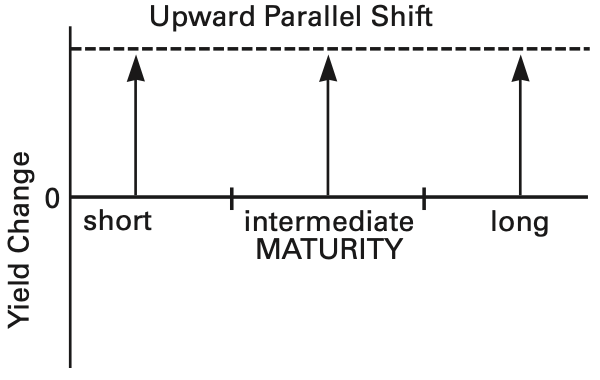
\includegraphics{1}
\end{frame}

\begin{frame}{Types de déplacement}
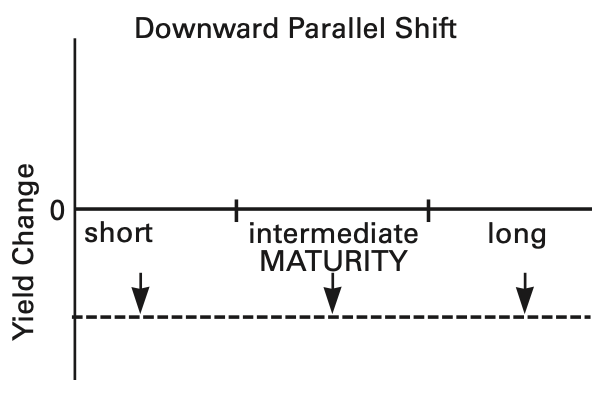
\includegraphics{2}
\end{frame}

\begin{frame}{Types de déplacement}
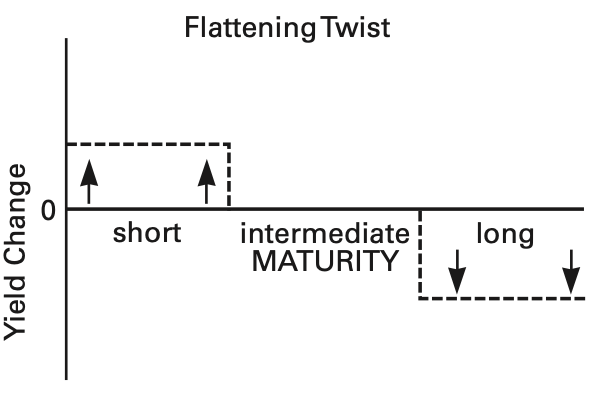
\includegraphics{3}
\end{frame}

\begin{frame}{Types de déplacement}
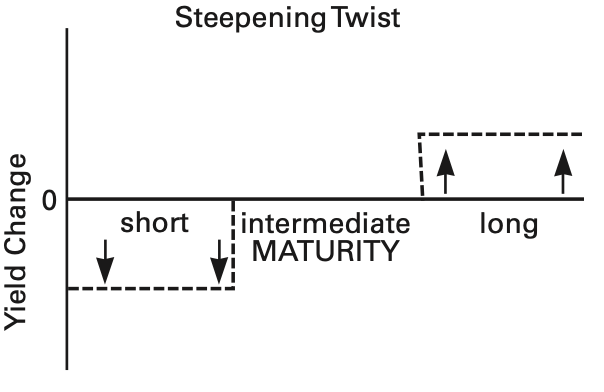
\includegraphics{4}
\end{frame}

\begin{frame}{Types de déplacement}
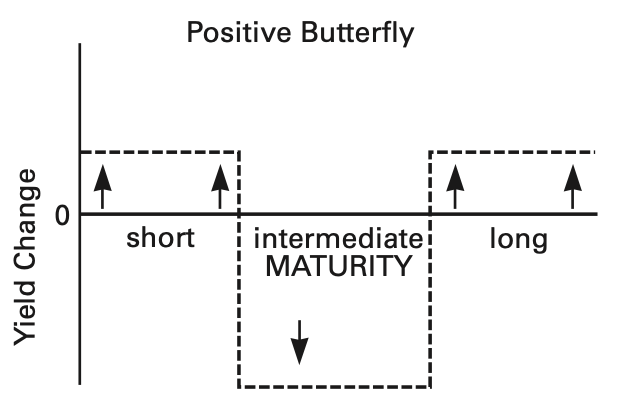
\includegraphics{5}
\end{frame}

\begin{frame}{Types de déplacement}
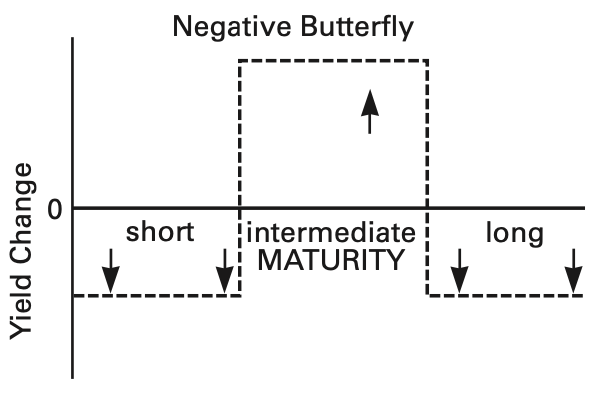
\includegraphics{6}
\end{frame}

\begin{frame}{Combinaisons de changements de courbe de rendement}
\begin{block}{Upward Shift/Flattening/Positive Butterfly}
Un déplacement à la hausse de la courbe des taux est souvent suivi par 
\begin{enumerate}[label=\arabic*)]
\item Flattening of the yield curve 
\item Positive Butterfly
\end{enumerate}
\end{block}
\begin{block}{Downward Shift/Steepening/Negative Butterfly}
Un déplacement à la baisse de la courbe des taux est souvent suivi par 
\begin{enumerate}[label=\arabic*)]
\item Steepening of the yield curve 
\item Negative Butterfly
\end{enumerate}
\end{block}
\end{frame}


\begin{frame}{Upward Shift/Flattening/Positive Butterfly}
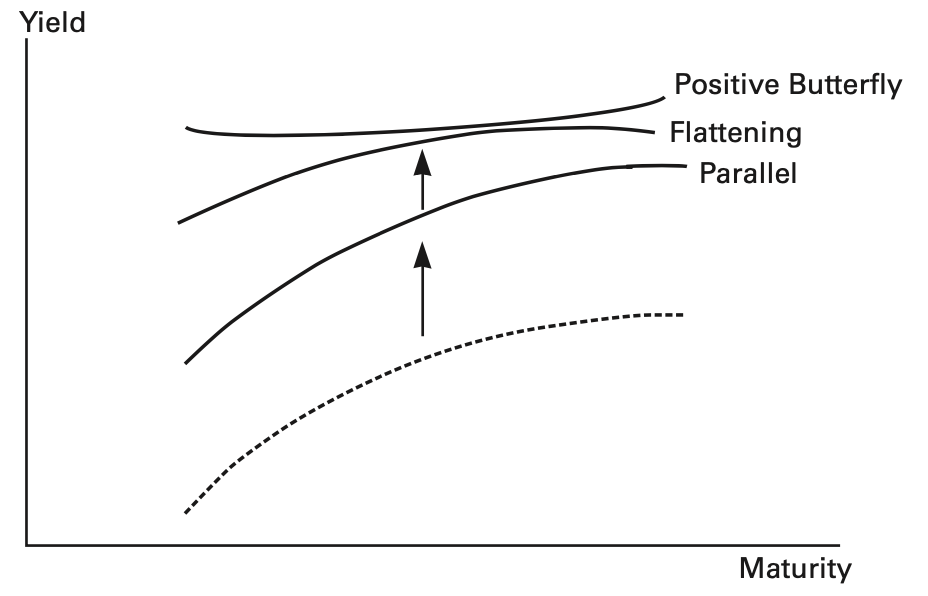
\includegraphics[scale=0.7]{7}
\end{frame}


\begin{frame}{Downward Shift/Steepening/Negative Butterfly}
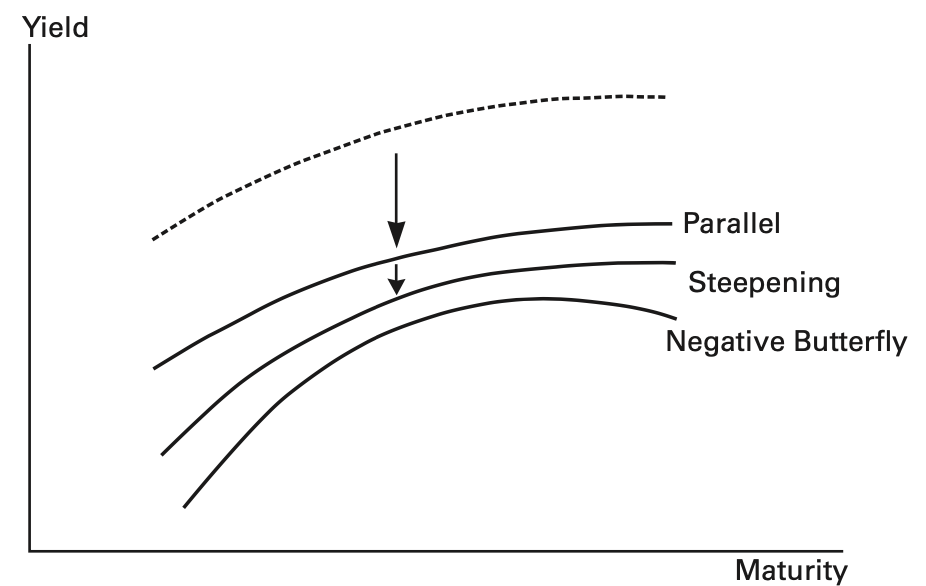
\includegraphics[scale=0.7]{8}
\end{frame}





\begin{frame}{Downward Shift/Steepening/Negative Butterfly}
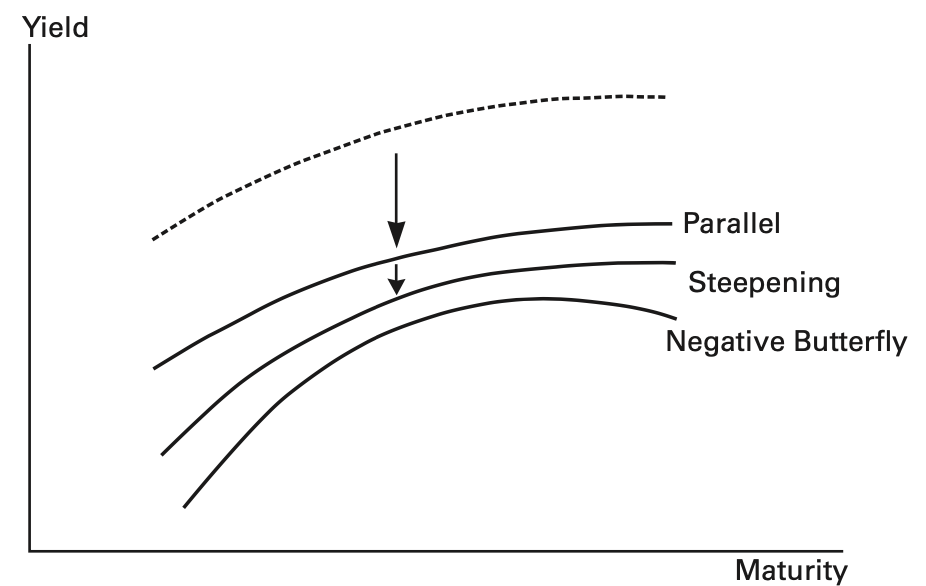
\includegraphics[scale=0.7]{8}
\end{frame}

\begin{frame}{Bullet strategy}
\begin{itemize}[label=\bullet]
\item Le portefeuille est construit de manière à ce que les échéances des titres du portefeuille soient fortement concentrées en un point de la courbe des taux.
\end{itemize}

\vspace{1cm}

\begin{center}
 \begin{tikzpicture}[snake=zigzag, line before snake = 5mm, line after snake = 5mm]
    % draw horizontal line   
    \draw (0,0) -- (9,0);

    % draw vertical lines
    \foreach \x in {0,1.5,3,4.5,6,7.5,9}
      \draw (\x cm,3pt) -- (\x cm,-3pt);
      
          \foreach \x in {2.8,2.9, 3,3.1,3.2}
      \draw (\x cm,30pt) -- (\x cm,-3pt);

    % draw nodes
    \draw (0,0) node[below=3pt] {$ 0 $} node[above=3pt] {$   $};
    \draw (1.5,0) node[below=3pt] {$ 5 $} node[above=3pt] {$  $};
    \draw (3,0) node[below=3pt] {$ 10 $} node[above=3pt] {$ $};
    \draw (4.5,0) node[below=3pt] {$ 15 $} node[above=3pt] {$  $};
    \draw (6,0) node[below=3pt] {$ 20 $} node[above=3pt] {$ $};
    \draw (7.5,0) node[below=3pt] {$ 25 $} node[above=3pt] {$  $};
    \draw (9,0) node[below=3pt] {$ 30 $} node[above=3pt] {$  $};
  \end{tikzpicture}
 \end{center}
\end{frame}

\begin{frame}{Barbell strategy}
\begin{itemize}[label=\bullet]
\item Les maturités des titres du portefeuille sont concentrées sur deux maturités extrêmes.
\end{itemize}

\vspace{1cm}

\begin{center}

 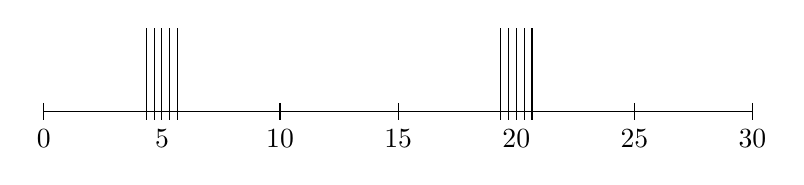
\begin{tikzpicture}[snake=zigzag, line before snake = 5mm, line after snake = 5mm]
    % draw horizontal line   
    \draw (0,0) -- (9,0);

    % draw vertical lines
    \foreach \x in {0,1.5,3,4.5,6,7.5,9}
      \draw (\x cm,3pt) -- (\x cm,-3pt);
      
          \foreach \x in {1.3,1.4,1.5,1.6,1.7,5.8,5.9,6,6.1,6.2}
      \draw (\x cm,30pt) -- (\x cm,-3pt);

    % draw nodes
    \draw (0,0) node[below=3pt] {$ 0 $} node[above=3pt] {$   $};
    \draw (1.5,0) node[below=3pt] {$ 5 $} node[above=3pt] {$  $};
    \draw (3,0) node[below=3pt] {$ 10 $} node[above=3pt] {$ $};
    \draw (4.5,0) node[below=3pt] {$ 15 $} node[above=3pt] {$  $};
    \draw (6,0) node[below=3pt] {$ 20 $} node[above=3pt] {$ $};
    \draw (7.5,0) node[below=3pt] {$ 25 $} node[above=3pt] {$  $};
    \draw (9,0) node[below=3pt] {$ 30 $} node[above=3pt] {$  $};
  \end{tikzpicture}
 \end{center}
\end{frame}

\begin{frame}{Ladder strategy}
\begin{itemize}[label=\bullet]
\item Le portefeuille est construit pour avoir des montants approximativement égaux à chaque échéance.
\end{itemize}

\vspace{1cm}

\begin{center}

 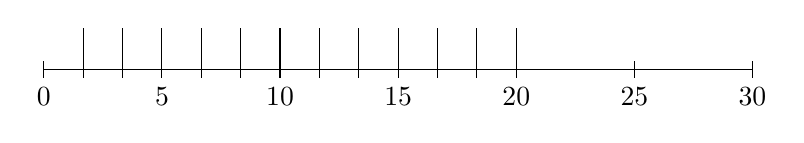
\begin{tikzpicture}[snake=zigzag, line before snake = 5mm, line after snake = 5mm]
    % draw horizontal line   
    \draw (0,0) -- (9,0);

    % draw vertical lines
    \foreach \x in {0,1.5,3,4.5,6,7.5,9}
      \draw (\x cm,3pt) -- (\x cm,-3pt);
      
          \foreach \x in {0.5,1,1.5,2,2.5,3,3.5,4,4.5,5,5.5,6}
      \draw (\x cm,15pt) -- (\x cm,-3pt);

    % draw nodes
    \draw (0,0) node[below=3pt] {$ 0 $} node[above=3pt] {$   $};
    \draw (1.5,0) node[below=3pt] {$ 5 $} node[above=3pt] {$  $};
    \draw (3,0) node[below=3pt] {$ 10 $} node[above=3pt] {$ $};
    \draw (4.5,0) node[below=3pt] {$ 15 $} node[above=3pt] {$  $};
    \draw (6,0) node[below=3pt] {$ 20 $} node[above=3pt] {$ $};
    \draw (7.5,0) node[below=3pt] {$ 25 $} node[above=3pt] {$  $};
    \draw (9,0) node[below=3pt] {$ 30 $} node[above=3pt] {$  $};
  \end{tikzpicture}
   \end{center}
\end{frame}

\begin{frame}{Changements de courbe de rendement et durée}
\begin{itemize}[label=\bullet]
\item La durée est une mesure de la sensibilité du prix d'une obligation ou de la valeur d'un portefeuille d'obligations suite aux variations des rendements du marché.
\end{itemize}
\begin{block}{Une obligation ayant une durée de 4}
Si les rendements du marché changent de 100 points de base (ou 1\%)\\
$\rightarrow$ Le prix de l'obligation changera d'environ 4\%.
\end{block}
\begin{block}{Un portefeuille d'obligations a une durée de 4}
Si les rendements du marché changent de 100 points de base (ou 1\%)\\
$\rightarrow$ La valeur du portefeuille changera d'environ 4\%.\\
$\rightarrow$ On suppose qu'il y a un déplacement parallèle de la courbe des taux.
\end{block}
\end{frame}

\begin{frame}{Obligations avec la même durée en dollars}
\begin{itemize}[label=\bullet]
\item Un gestionnaire de portefeuille détient des obligations X actuellement dans sont portefeuille.

\item Supposons que ce gestionnaire de portefeuille envisage d'échanger l'obligation X qu'il détient dans son portefeuille contre l'obligation Y
\item Si le gestionnaire de portefeuille souhaite avoir la même exposition aux taux d'intérêt (durée en dollars) pour l'obligation Y qu'elle a actuellement pour l'obligation X, elle achètera un montant à la valeur marchande de l'obligation Y avec la même durée en dollars.
\end{itemize}

\end{frame}

\begin{frame}{Obligations avec la même durée en dollars}
\begin{itemize}[label=\bullet]
\item $\$D_X=$ Durée en dollars par variation de 100 points de base du rendement de l'obligation X pour la valeur de marché de l'obligation X détenue.
\item $MD_Y=$ Durée modifiée de l'obligation Y
\item $MV_Y=$ Valeur de marché de l'obligation Y nécessaire pour obtenir la même durée en dollars que l'obligation X
\end{itemize}
\end{frame}

\begin{frame}{Obligations avec la même durée en dollars}
L'équation suivante définit la durée en dollars de l'obligation X comme étant égale à la durée en dollars de l'obligation Y:
\begin{align*}
\$D_X=\frac{MD_Y}{100}MV_Y
\end{align*}
On peut ensuite trouver:
\begin{align*}
MV_Y=\frac{\$ D_Y}{\frac{MD_Y}{100}}
\end{align*}
\end{frame}


\end{document}